\documentclass[12pt, titlepage]{article}

\usepackage{fullpage}
\usepackage[round]{natbib}
\usepackage{multirow}
\usepackage{booktabs}
\usepackage{tabularx}
\usepackage{graphicx}
\usepackage{float}
\usepackage{hyperref}
\hypersetup{
    colorlinks,
    citecolor=blue,
    filecolor=black,
    linkcolor=red,
    urlcolor=blue
}

\input{../../Comments}
%% Common Parts

\newcommand{\progname}{Baja Dynamics} % PUT YOUR PROGRAM NAME HERE
\newcommand{\authname}{Team \#17, Team Name
\\ Grace McKenna
\\ Travis Wing
\\ Cameron Dunn
\\ Kai Arseneau} % AUTHOR NAMES                  

\usepackage{hyperref}
    \hypersetup{colorlinks=true, linkcolor=blue, citecolor=blue, filecolor=blue,
                urlcolor=blue, unicode=false}
    \urlstyle{same}
                                


\newcounter{acnum}
\newcommand{\actheacnum}{AC\theacnum}
\newcommand{\acref}[1]{AC\ref{#1}}

\newcounter{ucnum}
\newcommand{\uctheucnum}{UC\theucnum}
\newcommand{\uref}[1]{UC\ref{#1}}

\newcounter{mnum}
\newcommand{\mthemnum}{M\themnum}
\newcommand{\mref}[1]{M\ref{#1}}

\begin{document}

\title{Module Guide for \progname{}} 
\author{\authname}
\date{\today}

\maketitle

\pagenumbering{roman}

\section{Revision History}

\begin{tabularx}{\textwidth}{p{3cm}p{2cm}X}
\toprule {\bf Date} & {\bf Version} & {\bf Notes}\\
\midrule
Date 1 & 1.0 & Notes\\
Date 2 & 1.1 & Notes\\
\bottomrule
\end{tabularx}

\newpage

\section{Reference Material}

This section records information for easy reference.

\subsection{Abbreviations and Acronyms}

\renewcommand{\arraystretch}{1.2}
\begin{tabular}{l l} 
  \toprule		
  \textbf{symbol} & \textbf{description}\\
  \midrule 
  AC & Anticipated Change\\
  DAG & Directed Acyclic Graph \\
  M & Module \\
  MG & Module Guide \\
  OS & Operating System \\
  R & Requirement\\
  SC & Scientific Computing \\
  SRS & Software Requirements Specification\\
  \progname & Explanation of program name\\
  UC & Unlikely Change \\
  \wss{etc.} & \wss{...}\\
  \bottomrule
\end{tabular}\\

\newpage

\tableofcontents

\listoftables

\listoffigures

\newpage

\pagenumbering{arabic}

\section{Introduction}

Decomposing a system into modules is a commonly accepted approach to developing
software.  A module is a work assignment for a programmer or programming
team~\citep{ParnasEtAl1984}.  We advocate a decomposition
based on the principle of information hiding~\citep{Parnas1972a}.  This
principle supports design for change, because the ``secrets'' that each module
hides represent likely future changes.  Design for change is valuable in SC,
where modifications are frequent, especially during initial development as the
solution space is explored.  

Our design follows the rules layed out by \citet{ParnasEtAl1984}, as follows:
\begin{itemize}
\item System details that are likely to change independently should be the
  secrets of separate modules.
\item Each data structure is implemented in only one module.
\item Any other program that requires information stored in a module's data
  structures must obtain it by calling access programs belonging to that module.
\end{itemize}

After completing the first stage of the design, the Software Requirements
Specification (SRS), the Module Guide (MG) is developed~\citep{ParnasEtAl1984}. The MG
specifies the modular structure of the system and is intended to allow both
designers and maintainers to easily identify the parts of the software.  The
potential readers of this document are as follows:

\begin{itemize}
\item New project members: This document can be a guide for a new project member
  to easily understand the overall structure and quickly find the
  relevant modules they are searching for.
\item Maintainers: The hierarchical structure of the module guide improves the
  maintainers' understanding when they need to make changes to the system. It is
  important for a maintainer to update the relevant sections of the document
  after changes have been made.
\item Designers: Once the module guide has been written, it can be used to
  check for consistency, feasibility, and flexibility. Designers can verify the
  system in various ways, such as consistency among modules, feasibility of the
  decomposition, and flexibility of the design.
\end{itemize}

The rest of the document is organized as follows. Section
\ref{SecChange} lists the anticipated and unlikely changes of the software
requirements. Section \ref{SecMH} summarizes the module decomposition that
was constructed according to the likely changes. Section \ref{SecConnection}
specifies the connections between the software requirements and the
modules. Section \ref{SecMD} gives a detailed description of the
modules. Section \ref{SecTM} includes two traceability matrices. One checks
the completeness of the design against the requirements provided in the SRS. The
other shows the relation between anticipated changes and the modules. Section
\ref{SecUse} describes the use relation between modules.

\section{Anticipated and Unlikely Changes} \label{SecChange}

This section lists possible changes to the system. According to the likeliness
of the change, the possible changes are classified into two
categories. Anticipated changes are listed in Section \ref{SecAchange}, and
unlikely changes are listed in Section \ref{SecUchange}.

\subsection{Anticipated Changes} \label{SecAchange}

Anticipated changes are the source of the information that is to be hidden
inside the modules. Ideally, changing one of the anticipated changes will only
require changing the one module that hides the associated decision. The approach
adapted here is called design for
change.

\begin{description}
  \item[\refstepcounter{acnum} \actheacnum \label{acHardware}:] The specific hardware on which the software is running.
  \item[\refstepcounter{acnum} \actheacnum \label{acInput}:] The format and structure of the initial input data.
  \item[\refstepcounter{acnum} \actheacnum \label{acEngineSimulator}:] The engine simulator implementation could be updated or replaced as new models or technologies become available.
  \item[\refstepcounter{acnum} \actheacnum \label{acExternalForces}:] External forces considered in the simulation could vary, depending on changes in design parameters or environmental considerations.
  \item[\refstepcounter{acnum} \actheacnum \label{acCVTSimulator}:] The CVT simulator implementation is likely change during the validation and verification (VnV) process.
  \item[\refstepcounter{acnum} \actheacnum \label{acVisualizations}:] The visualizations used, and their implementation could be updated to improve the user experience or to accommodate new features.
  \item[\refstepcounter{acnum} \actheacnum \label{acConstants}:] Constants used in the software could be updated based on changes to the car's physical design.
  \item[\refstepcounter{acnum} \actheacnum \label{acInputParameters}:] Input parameters for the system could change to include more parameters based on new requirements or to improve the accuracy of the simulation.
  \end{description}

\subsection{Unlikely Changes} \label{SecUchange}

The module design should be as general as possible. However, a general system is
more complex. Sometimes this complexity is not necessary. Fixing some design
decisions at the system architecture stage can simplify the software design. If
these decision should later need to be changed, then many parts of the design
will potentially need to be modified. Hence, it is not intended that these
decisions will be changed.

\begin{description}
  \item[\refstepcounter{ucnum} \uctheucnum \label{ucIO}:] Input/Output devices (Input: File and/or Keyboard, Output: File, Memory, and/or Screen).
  \item[\refstepcounter{ucnum} \uctheucnum \label{ucConstraints}:] Constraint parameters in our model/system will remain fixed and will not change.
  \item[\refstepcounter{ucnum} \uctheucnum \label{ucExcelRun}:] The simulation will always be an acceleration run, i.e. the car will always start from rest and accelerate.
\end{description}

\section{Module Hierarchy} \label{SecMH}

This section provides an overview of the module design. Modules are summarized
in a hierarchy decomposed by secrets in Table \ref{TblMH}. The modules listed
below, which are leaves in the hierarchy tree, are the modules that will
actually be implemented.

\begin{description}
  \item [\refstepcounter{mnum} \mthemnum \label{mHH}:] Hardware-Hiding Module
  \item [\refstepcounter{mnum} \mthemnum \label{mEngineSim}:] Engine Simulator Module
  \item [\refstepcounter{mnum} \mthemnum \label{mExternalForces}:] External Forces Module
  \item [\refstepcounter{mnum} \mthemnum \label{mPrimCVT}:] Primary CVT Module
  \item [\refstepcounter{mnum} \mthemnum \label{mSecCVT}:] Secondary CVT Module
  \item [\refstepcounter{mnum} \mthemnum \label{mInitialize}:] Initialize Module
  \item [\refstepcounter{mnum} \mthemnum \label{mODESolver}:] ODE Solver Module
  \item [\refstepcounter{mnum} \mthemnum \label{mMain}:] Main Module
  \item [\refstepcounter{mnum} \mthemnum \label{mPlayback}:] Playback Module
  \item [\refstepcounter{mnum} \mthemnum \label{mVisualizer}:] Visualizer Module
  \item [\refstepcounter{mnum} \mthemnum \label{mConstants}:] Constants Module
  \item [\refstepcounter{mnum} \mthemnum \label{mState}:] State Module
  \item [\refstepcounter{mnum} \mthemnum \label{mBCM}:] Backend Controller Module
  \item [\refstepcounter{mnum} \mthemnum \label{mGUI}:] GUI Module
  \item [\refstepcounter{mnum} \mthemnum \label{mFileOutput}:] File Output Module
  \item [\refstepcounter{mnum} \mthemnum \label{mComm}:] Communication Module
  \end{description}


\begin{table}[h!]
\centering
\begin{tabular}{p{0.3\textwidth} p{0.6\textwidth}}
\toprule
\textbf{Level 1} & \textbf{Level 2}\\
\midrule

{Hardware-Hiding Module} & ~ \\
\midrule

\multirow{7}{0.3\textwidth}{Behaviour-Hiding Module}
& Engine Simulator Module\\
& External Forces Module\\
& Primary CVT Module\\
& Secondary CVT Module\\
& Initialize Module\\
& ODE Solver Module\\
& Main Module\\ 
& Playback Module\\
& Visualizer Module\\
& Constants Module\\
& State Module\\
& Backend Controller Module\\
\midrule

\multirow{3}{0.3\textwidth}{Software Decision Module}
& GUI Module\\
& File Output Module\\
& Communication Module\\
\bottomrule

\end{tabular}
\caption{Module Hierarchy}
\label{TblMH}
\end{table}

\section{Connection Between Requirements and Design} \label{SecConnection}

The design of the system is intended to satisfy the requirements developed in
the SRS. In this stage, the system is decomposed into modules. The connection
between requirements and modules is listed in Table~\ref{TblRT}.

\wss{The intention of this section is to document decisions that are made
  ``between'' the requirements and the design.  To satisfy some requirements,
  design decisions need to be made.  Rather than make these decisions implicit,
  they are explicitly recorded here.  For instance, if a program has security
  requirements, a specific design decision may be made to satisfy those
  requirements with a password.}

\section{Module Decomposition} \label{SecMD}

Modules are decomposed according to the principle of ``information hiding''
proposed by \citet{ParnasEtAl1984}. The \emph{Secrets} field in a module
decomposition is a brief statement of the design decision hidden by the
module. The \emph{Services} field specifies \emph{what} the module will do
without documenting \emph{how} to do it. For each module, a suggestion for the
implementing software is given under the \emph{Implemented By} title. If the
entry is \emph{OS}, this means that the module is provided by the operating
system or by standard programming language libraries.  \emph{\progname{}} means the
module will be implemented by the \progname{} software.

Only the leaf modules in the hierarchy have to be implemented. If a dash
(\emph{--}) is shown, this means that the module is not a leaf and will not have
to be implemented.

\subsection{Hardware Hiding Modules (\mref{mHH})}

\begin{description}
\item[Secrets:]The data structure and algorithm used to implement the virtual
  hardware.
\item[Services:]Serves as a virtual hardware used by the rest of the
  system. This module provides the interface between the hardware and the
  software. So, the system can use it to display outputs or to accept inputs.
\item[Implemented By:] OS
\end{description}

\subsection{Behaviour-Hiding Module}

\begin{description}
\item[Secrets:]The contents of the required behaviors.
\item[Services:]Includes programs that provide externally visible behavior of
  the system as specified in the software requirements specification (SRS)
  documents. This module serves as a communication layer between the
  hardware-hiding module and the software decision module. The programs in this
  module will need to change if there are changes in the SRS.
\item[Implemented By:] --
\end{description}

\subsubsection{Engine Simulator Module (\mref{mEngineSim})}

\begin{description}
\item[Secrets:] The relationship between torque, RPM, and load in the engine's performance curve.
\item[Services:] Simulates engine behavior by generating torque based on input RPM, throttle position, and load conditions.
\item[Implemented By:] \progname{}
\item[Type of Module:] Abstract Object
\end{description}

\subsubsection{External Forces Module (\mref{mExternalForces})}

\begin{description}
\item[Secrets:] The equations for calculating gravity, air resistance, and rolling resistance forces acting on the vehicle.
\item[Services:] Computes the net external forces acting on the vehicle for given conditions like incline, speed, and drag coefficient.
\item[Implemented By:] \progname{}
\item[Type of Module:] Abstract Object
\end{description}

\subsubsection{Primary CVT Module (\mref{mPrimCVT})}

\begin{description}
\item[Secrets:] The dynamics of the primary CVT, including the relationship between clamping forces, belt ratios, and load transfer.
\item[Services:] Simulates the primary CVT's behavior under changing conditions by calculating primary clamping forces and belt ratios.
\item[Implemented By:] \progname{}
\item[Type of Module:] Abstract Object
\end{description}

\subsubsection{Secondary CVT Module (\mref{mSecCVT})}

\begin{description}
\item[Secrets:] The dynamics of the secondary CVT, including the relationship between clamping forces, belt ratios, and load transfer.
\item[Services:] Simulates the primary secondary CVT's behavior under changing conditions by calculating secondary clamping forces and belt ratios.
\item[Implemented By:] \progname{}
\item[Type of Module:] Abstract Object
\end{description}

\subsubsection{Initialize Module (\mref{mInitialize})}

\begin{description}
\item[Secrets:]The format and structure of the input data.
\item[Services:]Converts the input data into the initial state of the simulation.
\item[Implemented By:] \progname{}
\item[Type of Module:] Record
\end{description}


\subsubsection{ODE Solver Module (\mref{mODESolver})}

\begin{description}
\item[Secrets:] The numerical methods and parameters used by SciPy to solve ordinary differential equations.
\item[Services:] Solves the system of differential equations governing the CVT system's dynamics over time.
\item[Implemented By:] SciPy
\item[Type of Module:] Library
\end{description}

\subsubsection{Main Module (\mref{mMain})}

\begin{description}
\item[Secrets:] The orchestration of various modules to achieve the simulation flow.
\item[Services:] Manages the simulation's execution by calling the ODE solver, handling inputs/outputs, and coordinating between modules.
\item[Implemented By:] \progname{}
\item[Type of Module:] Abstract Object
\end{description}

\subsubsection{Playback Module (\mref{mPlayback})}

\begin{description}
\item[Secrets:] The format of simulation data and it's mapping to Unity playback mechanisms.
\item[Services:] Provides playback functionality by reading simulation data and rendering it in Unity.
\item[Implemented By:] \progname{}
\item[Type of Module:] Abstract Object
\end{description}

\subsubsection{Visualizer Module (\mref{mVisualizer})}

\begin{description}
\item[Secrets:] The graphical representation and rendering techniques used in Unity.
\item[Services:] Visualizes simulation results through charts, graphs, and 3D models, integrating data from various modules.
\item[Implemented By:] Unity
\item[Type of Module:] Abstract Object
\end{description}

\subsubsection{Constants Module (\mref{mConstants})}

\begin{description}
\item[Secrets:] The storage and retrieval of constant values like engine torque curves, car weight, and drag coefficients.
\item[Services:] Provides a centralized location for retrieving predefined constant values used across the simulation.
\item[Implemented By:] \progname{}
\item[Type of Module:] Library
\end{description}

\subsubsection{State Module (\mref{mState})}

\begin{description}
\item[Secrets:] The format of the system state.
\item[Services:] Stores and converts the system state between formats.
\item[Implemented By:] \progname{}
\item[Type of Module:] Record
\end{description}

\subsubsection{Backend Controller Module (\mref{mBCM})}

\begin{description}
\item[Secrets:] The orchestration of the backend simulation.
\item[Services:] Control the backend simulation.
\item[Implemented By:] \progname{}
\item[Type of Module:] Abstract Object
\end{description}



\subsection{Software Decision Module}

\begin{description}
\item[Secrets:] The design decision based on mathematical theorems, physical
  facts, or programming considerations. The secrets of this module are
  \emph{not} described in the SRS.
\item[Services:] Includes data structure and algorithms used in the system that
  do not provide direct interaction with the user. 
  % Changes in these modules are more likely to be motivated by a desire to
  % improve performance than by externally imposed changes.
\item[Implemented By:] --
\end{description}

\subsubsection{GUI Module (\mref{mGUI})}

\begin{description}
\item[Secrets:] The layout and design of the user interface.
\item[Services:] Displays simulation outputs to the user, enables interaction (e.g., input adjustments, playback controls), and visualizes simulation results in 3D and 2D formats.
\item[Implemented By:] \progname{}
\item[Type of Module:] Abstract Object
\end{description}

\subsubsection{File Output Module (\mref{mFileOutput})}

\begin{description}
\item[Secrets:] The format of the output data and the methods used for file serialization.
\item[Services:] Saves simulation results (e.g., graphs, raw data) into user-friendly formats like CSV or JSON for external use and analysis.
\item[Implemented By:] \progname{}
\item[Type of Module:] Library
\end{description}

\subsubsection{Communication Module (\mref{mComm})}

\begin{description}
\item[Secrets:] The protocol and serialization methods used for data exchange between Unity and the Python backend.
\item[Services:] Facilitates data transfer between the Unity-based GUI and the Python-based simulation modules, ensuring synchronization and integrity of inputs/outputs.
\item[Implemented By:] \progname{}
\item[Type of Module:] Abstract Object
\end{description}

\section{Traceability Matrix} \label{SecTM}

This section shows two traceability matrices: between the modules and the
requirements and between the modules and the anticipated changes.

% the table should use mref, the requirements should be named, use something
% like fref
\begin{table}[H]
\centering
\begin{tabular}{p{0.2\textwidth} p{0.6\textwidth}}
\toprule
\textbf{Req.} & \textbf{Modules}\\
\midrule
R1 & \mref{mPrimCVT}, \mref{mSecCVT}, \mref{mODESolver}, \mref{mConstants}\\
R2 & \mref{mExternalForces}, \mref{mConstants}\\
R3 & \mref{mExternalForces}, \mref{mConstants}\\
R4 & \mref{mExternalForces}, \mref{mConstants}\\
R5 & \mref{mPrimCVT}, \mref{mConstants}\\
R6 & \mref{mSecCVT}, \mref{mConstants}\\
R7 & \mref{mPrimCVT}, \mref{mSecCVT}, \mref{mConstants}\\
R8 & \mref{mPrimCVT}, \mref{mSecCVT}, \mref{mConstants}\\
R9 & \mref{mEngineSim}, \mref{mConstants}\\
R10 & \mref{mGUI}, \mref{mInitialize}\\
R11 & \mref{mGUI}, \mref{mInitialize}\\
R12 & \mref{mGUI}, \mref{mInitialize}\\
R13 & \mref{mVisualizer}, \mref{mPlayback}\\
R14 & \mref{mVisualizer}, \mref{mPlayback}\\
R15 & \mref{mVisualizer}, \mref{mPlayback}\\
R16 & \mref{mHH}\\
R17 & \mref{mHH}\\
\bottomrule
\end{tabular}
\caption{Trace Between Requirements and Modules}
\label{TblRT}
\end{table}

\begin{table}[H]
\centering
\begin{tabular}{p{0.2\textwidth} p{0.6\textwidth}}
\toprule
\textbf{AC} & \textbf{Modules}\\
\midrule
\acref{acHardware} & \mref{mHH}\\
\acref{acInput}\acref{acInputParameters} & \mref{mInitialize}\\
\acref{acEngineSimulator} & \mref{mEngineSim}\\
\acref{acExternalForces} & \mref{mExternalForces}\\
\acref{acCVTSimulator} & \mref{mPrimCVT}, \mref{mSecCVT},\\
\acref{acVisualizations} & \mref{mVisualizer}\\
\acref{acConstants} & \mref{mConstants}\\

\bottomrule
\end{tabular}
\caption{Trace Between Anticipated Changes and Modules}
\label{TblACT}
\end{table}

\section{Use Hierarchy Between Modules} \label{SecUse}

In this section, the uses' hierarchy between modules is
provided. \citet{Parnas1978} said of two programs A and B that A {\em uses} B if
correct execution of B may be necessary for A to complete the task described in
its specification. That is, A {\em uses} B if there exist situations in which
the correct functioning of A depends upon the availability of a correct
implementation of B.  Figure \ref{FigUH} illustrates the use relation between
the modules. It can be seen that the graph is a directed acyclic graph
(DAG). Each level of the hierarchy offers a testable and usable subset of the
system, and modules in the higher level of the hierarchy are essentially simpler
because they use modules from the lower levels.

\begin{figure}[H]
\centering
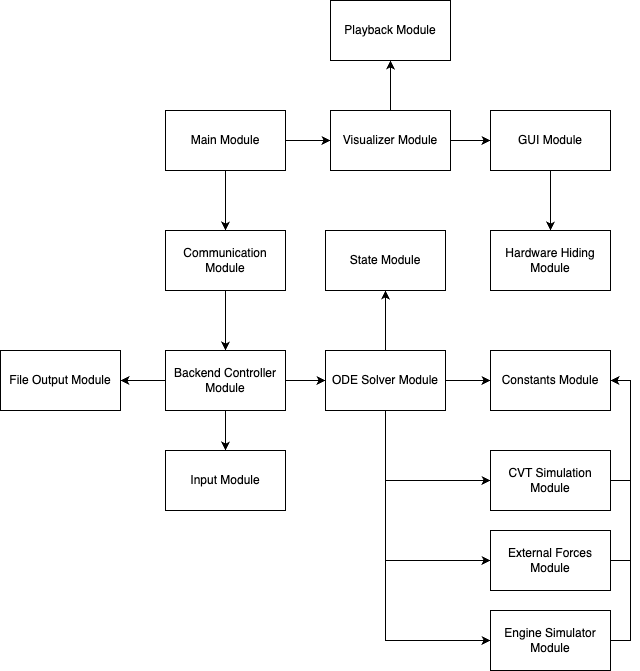
\includegraphics[width=0.7\textwidth]{moduleDrawing.drawio.png}
\caption{Use hierarchy among modules}
\label{FigUH}
\end{figure}

%\section*{References}

\section{User Interfaces}
\noindent Link to Figma:
\url{https://www.figma.com/design/REbQeg2EuDxgU07C6aS5Os/Capstone?node-id=0-1&t=0Ay7pkvwNLkEgVxE-1}
\\
\noindent Note that the screenshots of each interface can be seen in the Appendix of this document.

\noindent\wss{Design of user interface for software and hardware.  Attach an appendix if
needed. Drawings, Sketches, Figma}

\section{Design of Communication Protocols}
There are two main communication protocols used in the system.
One is for going from Unity to Python and the other is for going from Python to Unity.
Outside these two instances, the other modules' communication is handled through standard Unity or Python internal communication.

\subsection{Unity to Python}
The Unity from Python communication is handled through passing parameters.
Unity opens a terminal which calls the main Python script.
This call also includes all the parameters that are specified by the user.
These parameters are then received by the Python script and are used to run the simulation.

\subsection{Python to Unity}
The Python to Unity communication is handled through a CSV file.
After the simulation is run, the Python script writes the results to a CSV file.
Unity then reads from this CSV file and gets the results of the simulation.
This data is used to display the results of the simulation to the user.

\section{Timeline}

Rev 0 of the product is due by February 3rd, 2025. To ensure adequate time for any last-minute adjustments or unforeseen issues, the goal is to complete all tasks by February 1st, 2025.

\subsection*{Backend and Mathematical Model}
The backend and mathematical model are primarily the responsibility of Kai, with support from Cameron. The team aims to complete this work by January 27th, 2025. 

This includes:
\begin{enumerate}
\item Finalizing the CVT mathematical modules, which are critical to the product. Additionally, the engine and external forces modules, which are already complete, will be integrated into the system. This refers to modules \mref{mEngineSim}, \mref{mExternalForces}, and \mref{mCVT} and will be completed no later than January 22nd, 2025.
\item Following this, modules \mref{mODESolver}, \mref{mConstants}, \mref{mState}, and \mref{mBCM} will be developed. This will connect the previous work together to create a complete backend. This will be completed by January 25th, 2025.
\end{enumerate}

Initial validation and verification will also be conducted. These checks will include ensuring that values increase monotonically where expected, verifying the realism of generated values within the context of the problem, and performing quick automated tests that do not rely on realistic data. These steps will help ensure the robustness of the backend before integration. This will take up the remaining time.

\subsection*{Unity and User Interface (UI)}
The Unity and user interface components will be developed collaboratively by Travis and Grace. The deadline for this section is also January 27th, 2025. 

This includes:
\begin{enumerate}
\item Building the UI prototype based on the Figma design provided in Section 10 of the documentation along with basic output features. This refers to modules \mref{mGUI} and \mref{mFileOutput}  and will be completed by January 22nd, 2025.
\item Completing the Playback module (\mref{mPlayback}) by January 25th, 2025. This will involve using fed data from the backend with the Unity components to ensure that the simulation results are displayed accurately. This does not cover the communication module.
\end{enumerate}


This prototype will handle user input effectively and include visualizations such as 3D models, graphs, gauges, and other essential elements. These features are intended to provide an intuitive and visually engaging user experience. Initial testing of these will be done via early user feedback, ensuring simple bugs are caught and feedback can be acquired for later use. This will take the remaining time until January 27th, 2025.

\subsection*{Connecting the Components}
The integration of the backend and mathematical model with the Unity and UI components will involve all team members and will be completed by February 1st, 2025. This phase will ensure that the backend models connect seamlessly with their respective visualizations. Full playback functionality will also be implemented, allowing the system to operate as intended. This should complete module \mref{mComm}.

Team-wide testing will take place during this phase to identify and resolve any integration issues. Clear communication and collaboration between subteams will be crucial to ensure that all components function harmoniously.

\subsection*{Additional Notes}
All updates and task tracking will be managed through the project GitHub repository. The repository can be accessed at \url{https://github.com/gr812b/CVT-Simulator/issues}. Between January 27th and February 1st, 2025, effective communication between subteams will be vital to ensure the integration process proceeds smoothly. Team members are encouraged to check in regularly to verify that progress aligns with the established timeline.

\wss{Schedule of tasks and who is responsible}

\wss{You can point to GitHub if this information is included there}

\bibliographystyle {plainnat}
\bibliography{../../../refs/References}

\newpage
\section*{Appendix}
\begin{figure}[H]
  \begin{center}
   \includegraphics[width=0.7\textwidth]{{home.png}}
  \caption{Home Page }
  \label{Fig_Home} 
  \end{center}
  \end{figure}

\begin{figure}[H]
  \begin{center}
   \includegraphics[width=0.7\textwidth]{{inputs.png}}
  \caption{Inputs Page}
  \label{Fig_Inputs} 
  \end{center}
  \end{figure}

\begin{figure}[H]
  \begin{center}
   \includegraphics[width=0.7\textwidth]{{simulation.png}}
  \caption{Simulation Page}
  \label{Fig_Sim} 
  \end{center}
  \end{figure}


\end{document}